% GNUPLOT: LaTeX picture with Postscript
\documentclass{minimal}
% Set font size
\makeatletter
\def\@ptsize{1}
\InputIfFileExists{size11.clo}{}{%
   \GenericError{(gnuplot) \space\space\space\@spaces}{%
      Gnuplot Error: File `size11.clo' not found! Could not set font size%
   }{See the gnuplot documentation for explanation.%
   }{For using a font size a file `size<fontsize>.clo' has to exist.
        Falling back ^^Jto default fontsize 10pt.}%
  \def\@ptsize{0}
  \input{size10.clo}%
}%
\makeatother
% Load packages
\usepackage{calc}
\usepackage{graphicx}
\usepackage{color}
\makeatletter
% Select an appropriate default driver (from TeXLive graphics.cfg)
\begingroup
  \chardef\x=0 %
  % check pdfTeX
  \@ifundefined{pdfoutput}{}{%
    \ifcase\pdfoutput
    \else
      \chardef\x=1 %
    \fi
  }%
  % check VTeX
  \@ifundefined{OpMode}{}{%
    \chardef\x=2 %
  }%
\expandafter\endgroup
\ifcase\x
  % default case
  \PassOptionsToPackage{dvips}{geometry}
\or
  % pdfTeX is running in pdf mode
  \PassOptionsToPackage{pdftex}{geometry}
\else
  % VTeX is running
  \PassOptionsToPackage{vtex}{geometry}
\fi
\makeatother
% Set papersize
\usepackage[papersize={864.00bp,360.00bp},text={864.00bp,360.00bp}]{geometry}
% No page numbers and no paragraph indentation
\pagestyle{empty}
\setlength{\parindent}{0bp}%
% Load configuration file
\InputIfFileExists{gnuplot.cfg}{%
  \typeout{Using configuration file gnuplot.cfg}%
}{%
 \typeout{No configuration file gnuplot.cfg found.}%
}%
%
\begin{document}
\begingroup
  \makeatletter
  \providecommand\color[2][]{%
    \GenericError{(gnuplot) \space\space\space\@spaces}{%
      Package color not loaded in conjunction with
      terminal option `colourtext'%
    }{See the gnuplot documentation for explanation.%
    }{Either use 'blacktext' in gnuplot or load the package
      color.sty in LaTeX.}%
    \renewcommand\color[2][]{}%
  }%
  \providecommand\includegraphics[2][]{%
    \GenericError{(gnuplot) \space\space\space\@spaces}{%
      Package graphicx or graphics not loaded%
    }{See the gnuplot documentation for explanation.%
    }{The gnuplot epslatex terminal needs graphicx.sty or graphics.sty.}%
    \renewcommand\includegraphics[2][]{}%
  }%
  \providecommand\rotatebox[2]{#2}%
  \@ifundefined{ifGPcolor}{%
    \newif\ifGPcolor
    \GPcolortrue
  }{}%
  \@ifundefined{ifGPblacktext}{%
    \newif\ifGPblacktext
    \GPblacktexttrue
  }{}%
  % define a \g@addto@macro without @ in the name:
  \let\gplgaddtomacro\g@addto@macro
  % define empty templates for all commands taking text:
  \gdef\gplbacktext{}%
  \gdef\gplfronttext{}%
  \makeatother
  \ifGPblacktext
    % no textcolor at all
    \def\colorrgb#1{}%
    \def\colorgray#1{}%
  \else
    % gray or color?
    \ifGPcolor
      \def\colorrgb#1{\color[rgb]{#1}}%
      \def\colorgray#1{\color[gray]{#1}}%
      \expandafter\def\csname LTw\endcsname{\color{white}}%
      \expandafter\def\csname LTb\endcsname{\color{black}}%
      \expandafter\def\csname LTa\endcsname{\color{black}}%
      \expandafter\def\csname LT0\endcsname{\color[rgb]{1,0,0}}%
      \expandafter\def\csname LT1\endcsname{\color[rgb]{0,1,0}}%
      \expandafter\def\csname LT2\endcsname{\color[rgb]{0,0,1}}%
      \expandafter\def\csname LT3\endcsname{\color[rgb]{1,0,1}}%
      \expandafter\def\csname LT4\endcsname{\color[rgb]{0,1,1}}%
      \expandafter\def\csname LT5\endcsname{\color[rgb]{1,1,0}}%
      \expandafter\def\csname LT6\endcsname{\color[rgb]{0,0,0}}%
      \expandafter\def\csname LT7\endcsname{\color[rgb]{1,0.3,0}}%
      \expandafter\def\csname LT8\endcsname{\color[rgb]{0.5,0.5,0.5}}%
    \else
      % gray
      \def\colorrgb#1{\color{black}}%
      \def\colorgray#1{\color[gray]{#1}}%
      \expandafter\def\csname LTw\endcsname{\color{white}}%
      \expandafter\def\csname LTb\endcsname{\color{black}}%
      \expandafter\def\csname LTa\endcsname{\color{black}}%
      \expandafter\def\csname LT0\endcsname{\color{black}}%
      \expandafter\def\csname LT1\endcsname{\color{black}}%
      \expandafter\def\csname LT2\endcsname{\color{black}}%
      \expandafter\def\csname LT3\endcsname{\color{black}}%
      \expandafter\def\csname LT4\endcsname{\color{black}}%
      \expandafter\def\csname LT5\endcsname{\color{black}}%
      \expandafter\def\csname LT6\endcsname{\color{black}}%
      \expandafter\def\csname LT7\endcsname{\color{black}}%
      \expandafter\def\csname LT8\endcsname{\color{black}}%
    \fi
  \fi
    \setlength{\unitlength}{0.0500bp}%
    \ifx\gptboxheight\undefined%
      \newlength{\gptboxheight}%
      \newlength{\gptboxwidth}%
      \newsavebox{\gptboxtext}%
    \fi%
    \setlength{\fboxrule}{0.5pt}%
    \setlength{\fboxsep}{1pt}%
    \definecolor{tbcol}{rgb}{1,1,1}%
\begin{picture}(17280.00,7200.00)%
    \gplgaddtomacro\gplbacktext{%
      \csname LTb\endcsname%%
      \put(1188,4427){\makebox(0,0)[r]{\strut{}$0$}}%
      \put(1188,5093){\makebox(0,0)[r]{\strut{}$0.002$}}%
      \put(1188,5759){\makebox(0,0)[r]{\strut{}$0.004$}}%
      \put(1188,6426){\makebox(0,0)[r]{\strut{}$0.006$}}%
      \put(2083,4040){\makebox(0,0){\strut{}$-100$}}%
      \put(3036,4040){\makebox(0,0){\strut{}$-50$}}%
      \put(3990,4040){\makebox(0,0){\strut{}$0$}}%
      \put(4943,4040){\makebox(0,0){\strut{}$50$}}%
      \put(5896,4040){\makebox(0,0){\strut{}$100$}}%
      \put(1427,6834){\makebox(0,0)[l]{\strut{}\LARGE Trans. Ising}}%
      \put(1427,6459){\makebox(0,0)[l]{\strut{}\LARGE(a)}}%
      \put(1961,6459){\makebox(0,0)[l]{\strut{}\LARGE$\alpha=1.3$}}%
    }%
    \gplgaddtomacro\gplfronttext{%
      \csname LTb\endcsname%%
      \put(2319,5896){\makebox(0,0)[r]{\strut{}$t=600$}}%
      \csname LTb\endcsname%%
      \put(2319,5671){\makebox(0,0)[r]{\strut{}$t=800$}}%
      \csname LTb\endcsname%%
      \put(2319,5446){\makebox(0,0)[r]{\strut{}$t=1000$}}%
      \csname LTb\endcsname%%
      \put(2319,5221){\makebox(0,0)[r]{\strut{}$t=1200$}}%
      \csname LTb\endcsname%%
      \put(2319,4996){\makebox(0,0)[r]{\strut{}$t=1400$}}%
      \csname LTb\endcsname%%
      \put(319,5509){\rotatebox{-270.00}{\makebox(0,0){\strut{}\LARGE$t^{5/8} C(n,t)$}}}%
      \put(3989,3710){\makebox(0,0){\strut{}\LARGE$ n/t^{5/8} $}}%
    }%
    \gplgaddtomacro\gplbacktext{%
      \csname LTb\endcsname%%
      \put(5570,5669){\makebox(0,0)[r]{\strut{}$0$}}%
      \put(5570,6086){\makebox(0,0)[r]{\strut{}$0.001$}}%
      \put(5570,6502){\makebox(0,0)[r]{\strut{}$0.002$}}%
      \put(5570,6919){\makebox(0,0)[r]{\strut{}$0.003$}}%
      \put(6131,5324){\makebox(0,0){\strut{}$-200$}}%
      \put(6607,5324){\makebox(0,0){\strut{}$-100$}}%
      \put(7084,5324){\makebox(0,0){\strut{}$0$}}%
      \put(7561,5324){\makebox(0,0){\strut{}$100$}}%
      \put(8037,5324){\makebox(0,0){\strut{}$200$}}%
      \put(5840,6969){\makebox(0,0)[l]{\strut{}\Large$C(n,t)$}}%
    }%
    \gplgaddtomacro\gplfronttext{%
      \csname LTb\endcsname%%
      \put(7084,4994){\makebox(0,0){\strut{}\Large$n$}}%
    }%
    \gplgaddtomacro\gplbacktext{%
      \csname LTb\endcsname%%
      \put(9960,4416){\makebox(0,0)[r]{\strut{}$0$}}%
      \put(9960,4937){\makebox(0,0)[r]{\strut{}$0.001$}}%
      \put(9960,5457){\makebox(0,0)[r]{\strut{}$0.002$}}%
      \put(9960,5978){\makebox(0,0)[r]{\strut{}$0.003$}}%
      \put(9960,6499){\makebox(0,0)[r]{\strut{}$0.004$}}%
      \put(10855,4040){\makebox(0,0){\strut{}$-100$}}%
      \put(11808,4040){\makebox(0,0){\strut{}$-50$}}%
      \put(12762,4040){\makebox(0,0){\strut{}$0$}}%
      \put(13715,4040){\makebox(0,0){\strut{}$50$}}%
      \put(14668,4040){\makebox(0,0){\strut{}$100$}}%
      \put(10199,6834){\makebox(0,0)[l]{\strut{}\LARGE XYZ}}%
      \put(10199,6459){\makebox(0,0)[l]{\strut{}\LARGE(c)}}%
      \put(10733,6459){\makebox(0,0)[l]{\strut{}\LARGE$\alpha=1.3$}}%
    }%
    \gplgaddtomacro\gplfronttext{%
      \csname LTb\endcsname%%
      \put(11091,5896){\makebox(0,0)[r]{\strut{}$t=720$}}%
      \csname LTb\endcsname%%
      \put(11091,5671){\makebox(0,0)[r]{\strut{}$t=960$}}%
      \csname LTb\endcsname%%
      \put(11091,5446){\makebox(0,0)[r]{\strut{}$t=1200$}}%
      \csname LTb\endcsname%%
      \put(11091,5221){\makebox(0,0)[r]{\strut{}$t=1440$}}%
      \csname LTb\endcsname%%
      \put(11091,4996){\makebox(0,0)[r]{\strut{}$t=1680$}}%
      \csname LTb\endcsname%%
      \put(9091,5509){\rotatebox{-270.00}{\makebox(0,0){\strut{}\LARGE$t^{5/8} C(n,t)$}}}%
      \put(12761,3710){\makebox(0,0){\strut{}\LARGE$ n/t^{5/8} $}}%
    }%
    \gplgaddtomacro\gplbacktext{%
      \csname LTb\endcsname%%
      \put(14383,5676){\makebox(0,0)[r]{\strut{}$0$}}%
      \put(14383,6006){\makebox(0,0)[r]{\strut{}$0.0005$}}%
      \put(14383,6336){\makebox(0,0)[r]{\strut{}$0.001$}}%
      \put(14383,6665){\makebox(0,0)[r]{\strut{}$0.0015$}}%
      \put(14383,6995){\makebox(0,0)[r]{\strut{}$0.002$}}%
      \put(14944,5324){\makebox(0,0){\strut{}$-200$}}%
      \put(15420,5324){\makebox(0,0){\strut{}$-100$}}%
      \put(15897,5324){\makebox(0,0){\strut{}$0$}}%
      \put(16374,5324){\makebox(0,0){\strut{}$100$}}%
      \put(16850,5324){\makebox(0,0){\strut{}$200$}}%
      \put(14653,6969){\makebox(0,0)[l]{\strut{}\Large$C(n,t)$}}%
    }%
    \gplgaddtomacro\gplfronttext{%
      \csname LTb\endcsname%%
      \put(15897,4994){\makebox(0,0){\strut{}\Large$n$}}%
    }%
    \gplgaddtomacro\gplbacktext{%
      \csname LTb\endcsname%%
      \put(1188,1049){\makebox(0,0)[r]{\strut{}$0$}}%
      \put(1188,1725){\makebox(0,0)[r]{\strut{}$0.002$}}%
      \put(1188,2400){\makebox(0,0)[r]{\strut{}$0.004$}}%
      \put(1188,3076){\makebox(0,0)[r]{\strut{}$0.006$}}%
      \put(2083,660){\makebox(0,0){\strut{}$-100$}}%
      \put(3036,660){\makebox(0,0){\strut{}$-50$}}%
      \put(3990,660){\makebox(0,0){\strut{}$0$}}%
      \put(4943,660){\makebox(0,0){\strut{}$50$}}%
      \put(5896,660){\makebox(0,0){\strut{}$100$}}%
      \put(1427,3455){\makebox(0,0)[l]{\strut{}\LARGE Trans. Ising}}%
      \put(1427,3080){\makebox(0,0)[l]{\strut{}\LARGE(b)}}%
      \put(1961,3080){\makebox(0,0)[l]{\strut{}\LARGE$\alpha=1.6$}}%
    }%
    \gplgaddtomacro\gplfronttext{%
      \csname LTb\endcsname%%
      \put(2319,2517){\makebox(0,0)[r]{\strut{}$t=1200$}}%
      \csname LTb\endcsname%%
      \put(2319,2292){\makebox(0,0)[r]{\strut{}$t=1600$}}%
      \csname LTb\endcsname%%
      \put(2319,2067){\makebox(0,0)[r]{\strut{}$t=2000$}}%
      \csname LTb\endcsname%%
      \put(2319,1842){\makebox(0,0)[r]{\strut{}$t=2400$}}%
      \csname LTb\endcsname%%
      \put(2319,1617){\makebox(0,0)[r]{\strut{}$t=2800$}}%
      \csname LTb\endcsname%%
      \put(319,2130){\rotatebox{-270.00}{\makebox(0,0){\strut{}\LARGE$t^{1/2} C(n,t)$}}}%
      \put(3989,330){\makebox(0,0){\strut{}\LARGE$ n/t^{1/2} $}}%
    }%
    \gplgaddtomacro\gplbacktext{%
      \csname LTb\endcsname%%
      \put(5570,2192){\makebox(0,0)[r]{\strut{}$0$}}%
      \put(5570,2544){\makebox(0,0)[r]{\strut{}$0.001$}}%
      \put(5570,2896){\makebox(0,0)[r]{\strut{}$0.002$}}%
      \put(5570,3248){\makebox(0,0)[r]{\strut{}$0.003$}}%
      \put(5570,3600){\makebox(0,0)[r]{\strut{}$0.004$}}%
      \put(6131,1796){\makebox(0,0){\strut{}$-200$}}%
      \put(6607,1796){\makebox(0,0){\strut{}$-100$}}%
      \put(7084,1796){\makebox(0,0){\strut{}$0$}}%
      \put(7561,1796){\makebox(0,0){\strut{}$100$}}%
      \put(8037,1796){\makebox(0,0){\strut{}$200$}}%
      \put(5840,3442){\makebox(0,0)[l]{\strut{}\Large$C(n,t)$}}%
    }%
    \gplgaddtomacro\gplfronttext{%
      \csname LTb\endcsname%%
      \put(7084,1466){\makebox(0,0){\strut{}\Large$n$}}%
    }%
    \gplgaddtomacro\gplbacktext{%
      \csname LTb\endcsname%%
      \put(9960,1015){\makebox(0,0)[r]{\strut{}$0$}}%
      \put(9960,1691){\makebox(0,0)[r]{\strut{}$0.001$}}%
      \put(9960,2366){\makebox(0,0)[r]{\strut{}$0.002$}}%
      \put(9960,3042){\makebox(0,0)[r]{\strut{}$0.003$}}%
      \put(10855,660){\makebox(0,0){\strut{}$-100$}}%
      \put(11808,660){\makebox(0,0){\strut{}$-50$}}%
      \put(12762,660){\makebox(0,0){\strut{}$0$}}%
      \put(13715,660){\makebox(0,0){\strut{}$50$}}%
      \put(14668,660){\makebox(0,0){\strut{}$100$}}%
      \put(10199,3455){\makebox(0,0)[l]{\strut{}\LARGE XYZ}}%
      \put(10199,3080){\makebox(0,0)[l]{\strut{}\LARGE(d)}}%
      \put(10733,3080){\makebox(0,0)[l]{\strut{}\LARGE$\alpha=1.6$}}%
    }%
    \gplgaddtomacro\gplfronttext{%
      \csname LTb\endcsname%%
      \put(11091,2517){\makebox(0,0)[r]{\strut{}$t=1200$}}%
      \csname LTb\endcsname%%
      \put(11091,2292){\makebox(0,0)[r]{\strut{}$t=1600$}}%
      \csname LTb\endcsname%%
      \put(11091,2067){\makebox(0,0)[r]{\strut{}$t=2000$}}%
      \csname LTb\endcsname%%
      \put(11091,1842){\makebox(0,0)[r]{\strut{}$t=2400$}}%
      \csname LTb\endcsname%%
      \put(11091,1617){\makebox(0,0)[r]{\strut{}$t=2800$}}%
      \csname LTb\endcsname%%
      \put(9091,2130){\rotatebox{-270.00}{\makebox(0,0){\strut{}\LARGE$t^{1/2} C(n,t)$}}}%
      \put(12761,330){\makebox(0,0){\strut{}\LARGE$n/t^{1/2}$}}%
    }%
    \gplgaddtomacro\gplbacktext{%
      \csname LTb\endcsname%%
      \put(14383,2160){\makebox(0,0)[r]{\strut{}$0$}}%
      \put(14383,2520){\makebox(0,0)[r]{\strut{}$0.0005$}}%
      \put(14383,2880){\makebox(0,0)[r]{\strut{}$0.001$}}%
      \put(14383,3240){\makebox(0,0)[r]{\strut{}$0.0015$}}%
      \put(14383,3600){\makebox(0,0)[r]{\strut{}$0.002$}}%
      \put(14944,1796){\makebox(0,0){\strut{}$-200$}}%
      \put(15420,1796){\makebox(0,0){\strut{}$-100$}}%
      \put(15897,1796){\makebox(0,0){\strut{}$0$}}%
      \put(16374,1796){\makebox(0,0){\strut{}$100$}}%
      \put(16850,1796){\makebox(0,0){\strut{}$200$}}%
      \put(14653,3442){\makebox(0,0)[l]{\strut{}\Large$C(n,t)$}}%
    }%
    \gplgaddtomacro\gplfronttext{%
      \csname LTb\endcsname%%
      \put(15897,1466){\makebox(0,0){\strut{}\Large$n$}}%
    }%
    \gplbacktext
    \put(0,0){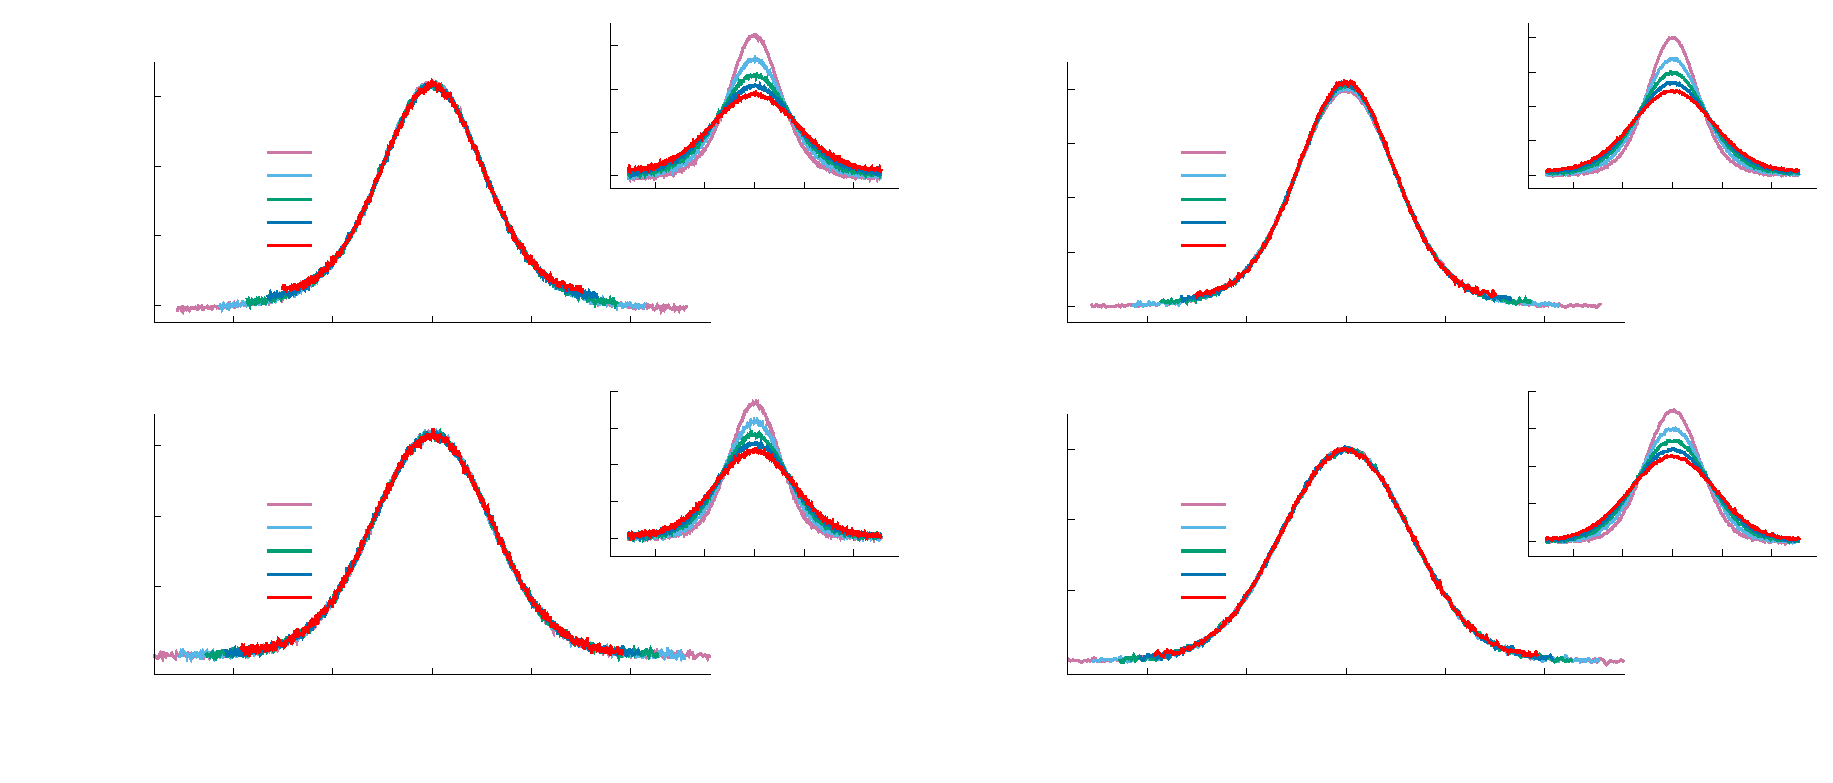
\includegraphics[width={864.00bp},height={360.00bp}]{fig3-inc}}%
    \gplfronttext
  \end{picture}%
\endgroup
\end{document}
